\documentclass{beamer}
\usepackage{graphicx} % Required for inserting images

\usepackage[utf8]{inputenc}
\usepackage[T1]{fontenc}
\usepackage{lmodern}
\usepackage{amsmath,amssymb}
\usepackage{microtype}
\usepackage{ellipsis}
%\usepackage[ngerman]{babel}
\let\openbox\undefined
\usepackage{mathtools}
\usepackage{enumitem}
\let\openbox\undefined
\usepackage{amsthm}
\usepackage{thmtools}
\usepackage{graphicx}
\usepackage{stmaryrd}
\usepackage{tikz}
\usetikzlibrary{positioning}
\usepackage{algpseudocode}
\usepackage[absolute,overlay]{textpos}
\usepackage{url}
\usepackage[
backend=biber,
style=numeric,
]{biblatex}
\addbibresource{references.bib}
\usepackage[normalem]{ulem}
\usepackage{verbatim}
\usepackage{subcaption} % allow for subfigures

\declaretheoremstyle[
    headpunct=,
    spacebelow=2em,
    spaceabove=1em,
    postheadspace=\newline,
    ]{aufgabe}
\declaretheorem[style=aufgabe]{aufgabe}
\numberwithin{equation}{aufgabe}
\addtolength\jot{1ex}

\newtheorem{proposition}{Proposition}
\renewcommand\qedsymbol{$\square$}

\newcommand\R{\mathbb R}
\newcommand\Z{\mathbb Z}
\newcommand\N{\mathbb N}
\newcommand\C{\mathbb C}
\newcommand{\Q}{\mathbb Q}
\newcommand{\F}{\mathbb{F}}
\newcommand{\ass}{\underline{Assume:}  }
\newcommand{\zz}{\underline{t.s.:}  }

\usetheme[compress]{Berlin}
\setbeamertemplate{footline}[frame number]{}
\setbeamertemplate{navigation symbols}{}
\setbeamertemplate{footline}{}

\makeatletter
\beamer@theme@subsectionfalse%
\makeatother


\title{The GAPic Package}
\subtitle{}
\author{Lukas Schnelle}
\date{GAPDays Spring 2024}

\begin{document}

% remove dots on first slide
\frame[plain]{\titlepage}

\section{Definitions}
\begin{frame}
    \begin{definition}\label{def:triangular-comp}
    	Let $X_0$ ("vertices"), $X_1$ ("edges") and $X_2$ ("faces") subsets of $\N_0$ and $\prec$ a symmetric relation between the sets called \emph{incidence}. \pause \\
    	We call $(\prec, X_0, X_1, X_2)$ \emph{triangular complex} if
    	\begin{enumerate}[label=(\roman*)] \pause 
    		\item $\prec$ is transitive, i.e. $\forall v \in X_0, e \in X_1, f \in X_2$:
    		$$(v \prec e) \wedge (e \prec f) \Rightarrow v \prec f$$ \vspace{-15px} \pause
    		\item $\forall e \in X_1 \exists \, f \in X_2$ such that $e \prec f$ \pause 
    		\item \pause $\forall e \in X_1 \exists !\,  v_1 \neq v_2 \in X_0$ such that $v_1, v_2 \prec e$ \pause 
    		\item $\forall f \in X_2 \exists ! \, v_1 \neq v_2 \neq v_3 \in X_0$ such that $v_1, v_2, v_3 \prec f$ \pause 
            \item $\forall f \in X_2 \exists ! \, e_1 \neq e_2 \neq e_3 \in X_1$ such that $e_1, e_2, e_3 \prec f$ \pause 
    	\end{enumerate}
    \end{definition}
\end{frame}

\begin{frame}
    \begin{definition}
        Let $(\prec, X_0, X_1, X_2)$ be a triangular complex.\\
        Then we call $(\prec, X_0, X_1, X_2)$ \emph{simplicial surface} if \pause
        \begin{enumerate}[label=(\roman*)]
            \item $\forall e \in X_1 : | \{ f \in X_2 \mid e \prec f \} | \leq 2 $ 
            \item $\forall v \in X_0 : def(v) \coloneqq | \{ f \in X_2 \mid v \prec f \} | < \infty$ 
            \item $\forall v \in X_0: $ there is an ordering of $e_1, f_1, \dots, e_{deg(v)}, f_{deg(v)} \prec v$ such that 
            $$
                e_1 \prec f_1 \prec e_2 \prec f_2 \prec \dots \prec f_{deg(v)} \prec e_{deg(v)}
            $$
            with $e_1 = e_{deg}(v)$ if (i) is an equality.\pause
        \end{enumerate} 
        Condition (iii) is called the \emph{umbrella condition}.
    \end{definition}
\end{frame}

\begin{frame}
    \begin{example}
        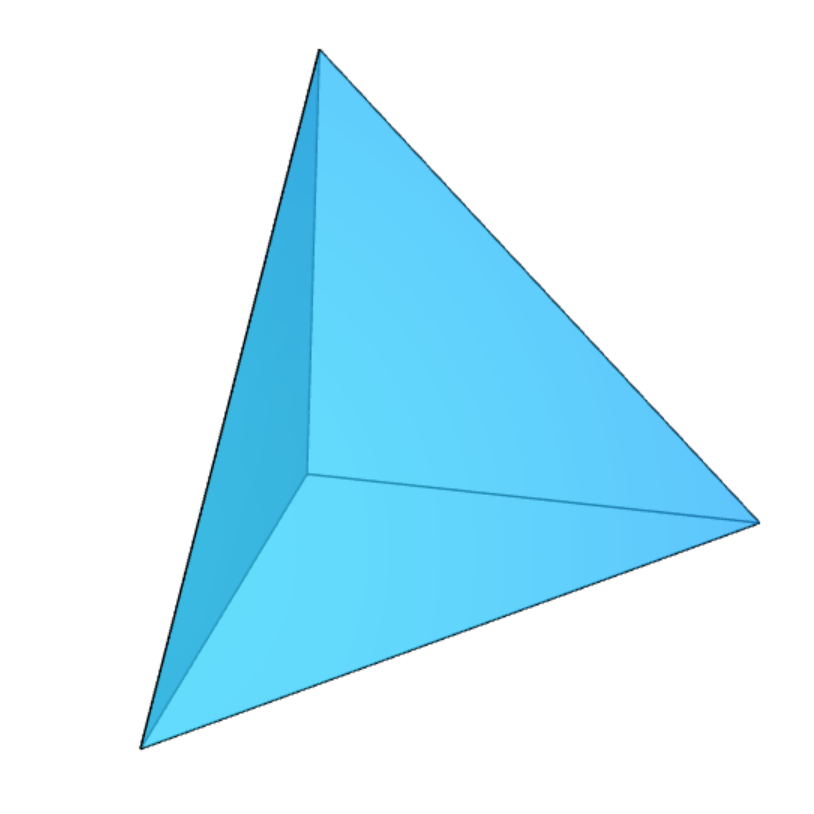
\includegraphics[width=0.48\textwidth]{images/tet.png}
        \uncover<3->{
        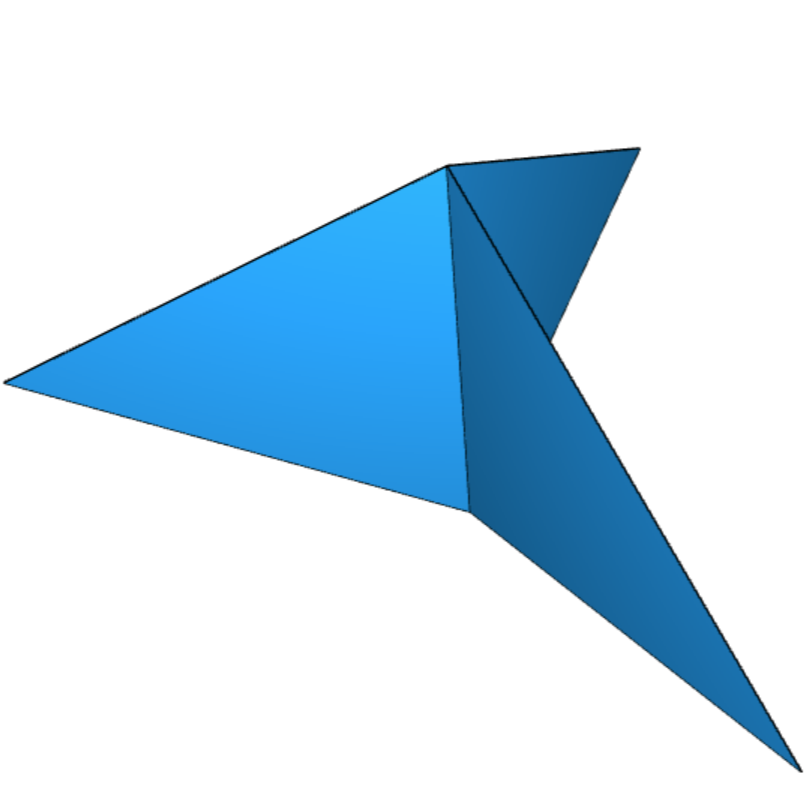
\includegraphics[width=0.48\textwidth]{images/complex3.png}}\\
        \uncover<2->{Simplicial Surface} \hspace{68pt} \uncover<4>{Triangular complex}
    \end{example}
\end{frame}

\begin{frame}
    \begin{definition}\label{def:embedding}
        Let $(\prec, X_0, X_1, X_2)$ be a triangular complex. \\ \pause
        Then we define an \emph{embedding} of $(\prec, X_0, X_1, X_2)$ as a map 
        $$c: X_0 \to \R^3$$ \pause
        The image of $v \in X_0$ is called \emph{coordinate of $v$}.
    \end{definition}
    \pause
    \begin{example}
        \vspace{-5px}
        \begin{figure}[H]
            \centering
            \begin{subfigure}[t]{0.3\textwidth}
                \centering
                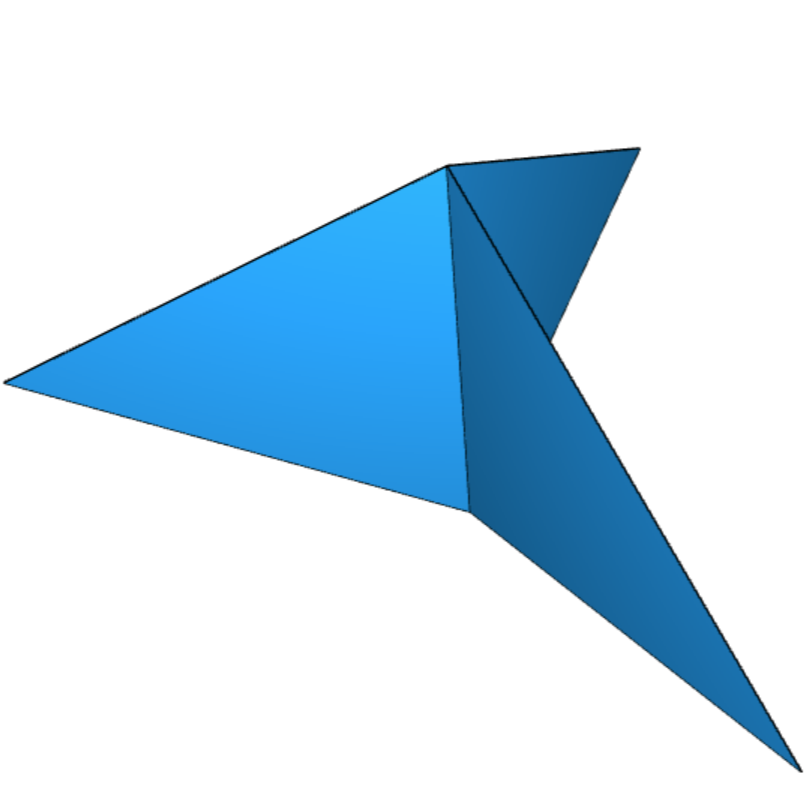
\includegraphics[width=0.9\textwidth]{images/complex3.png} 
                Embedded triangular complex
            \end{subfigure}
            \hspace{50pt}
            \pause
            \begin{subfigure}[t]{0.3\textwidth}
                \centering
                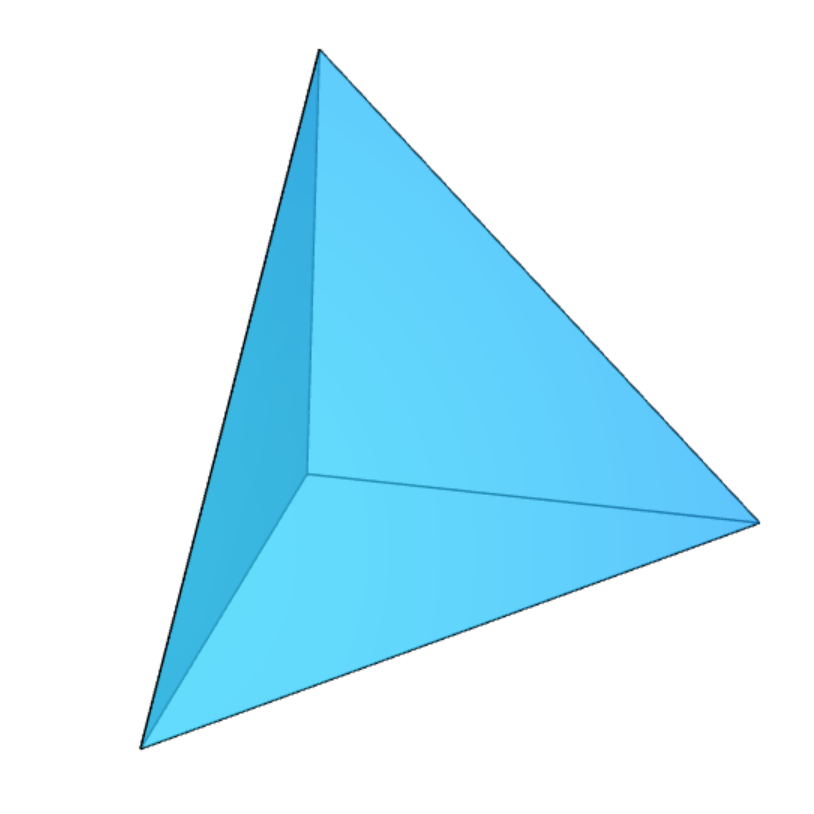
\includegraphics[width=0.9\textwidth]{images/tet.png}
                Embedded simplicial surface
            \end{subfigure}
        \end{figure}
        \vspace{-5px}
    \end{example}
\end{frame}

\section{SimplicialSurfaces Package}
\begin{frame}{Simplicial Surfaces Package}
    \begin{itemize}[label=-]
        \item Has functionality for displaying simplicial surfaces
        \begin{itemize}[label=-]
            \item Generates a .html file
            \item Uses three.js
        \end{itemize}
    \end{itemize}
    \pause
    \begin{example}[Number 2.1 and 2.2 from \cite{ico}]
        \centering
        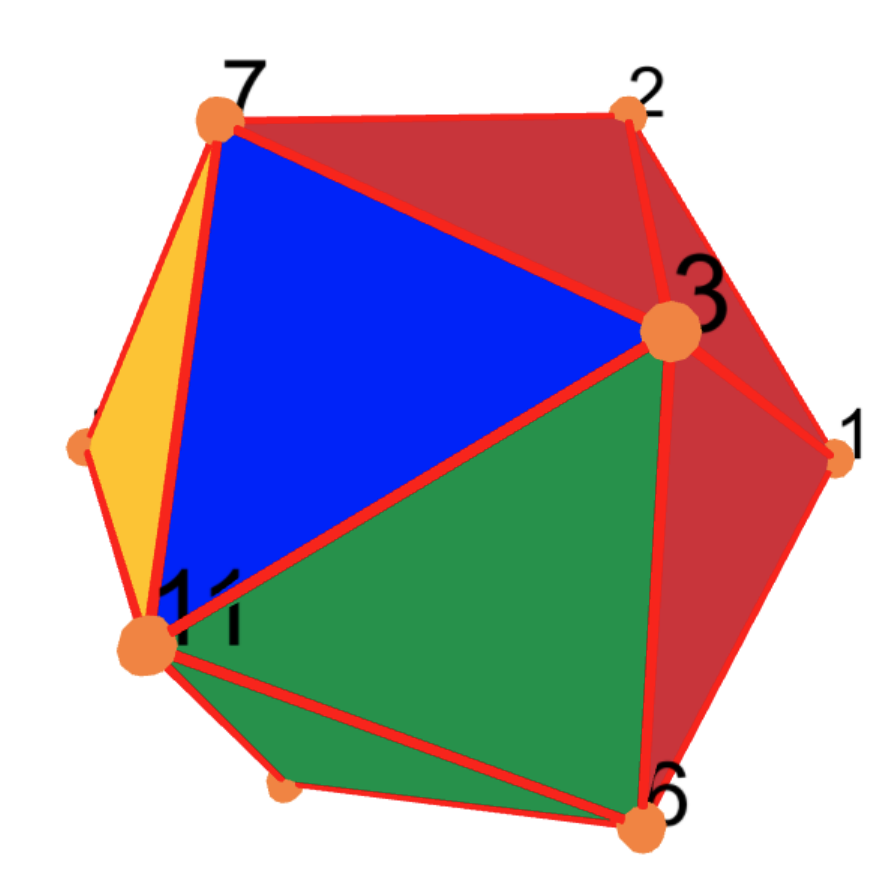
\includegraphics[width=0.4\textwidth]{images/ico-old.png}
        \hspace{10px}
        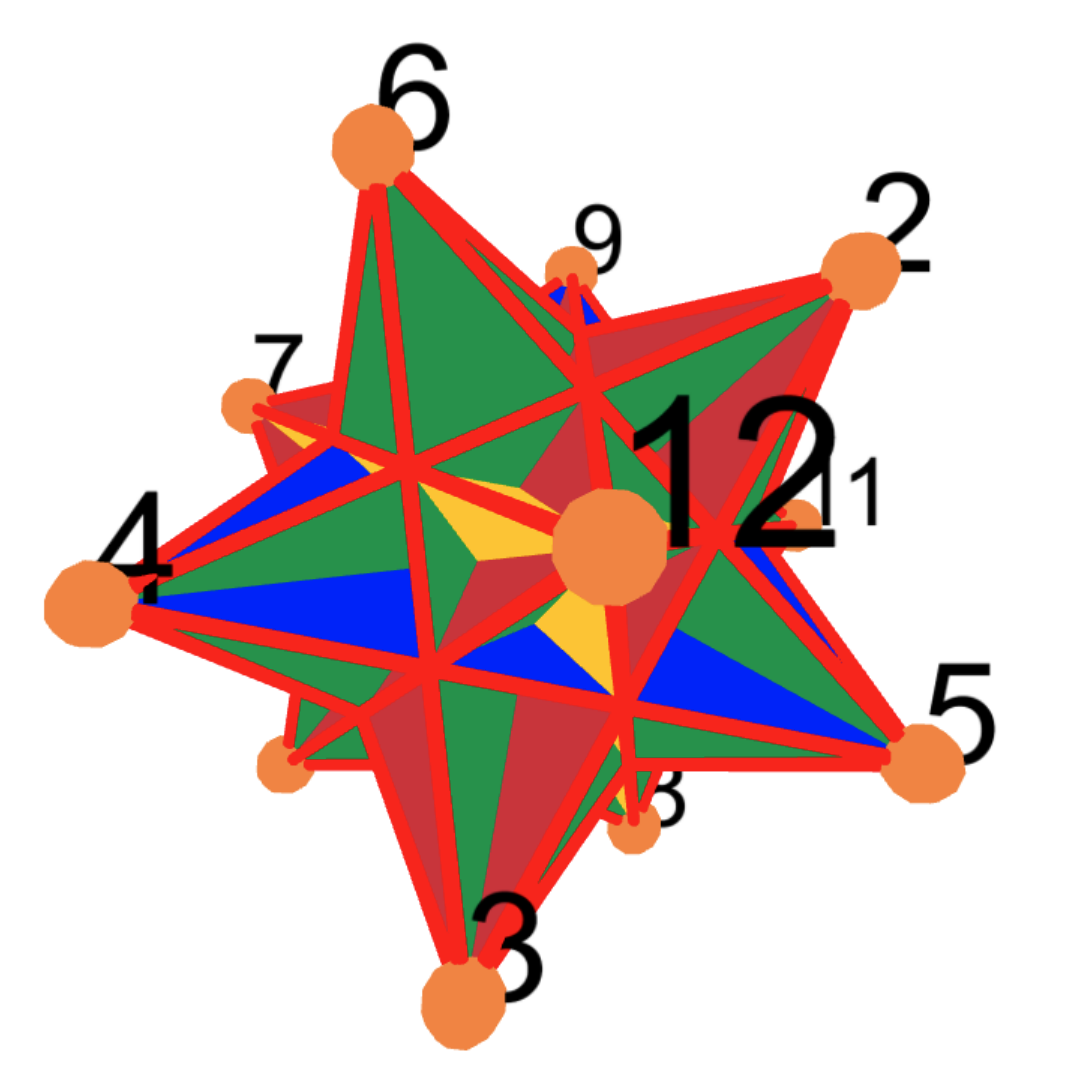
\includegraphics[width=0.4\textwidth]{images/ico2-1_old.png}
    \end{example}
\end{frame}

\begin{frame}
    \begin{exampleblock}{Fachpraktikum}
        Was a project with the goal to improve the visualizations by adding shading/local lighting.
        \pause \\
        After some work it turns out: central class used in implementation is deprecated.
        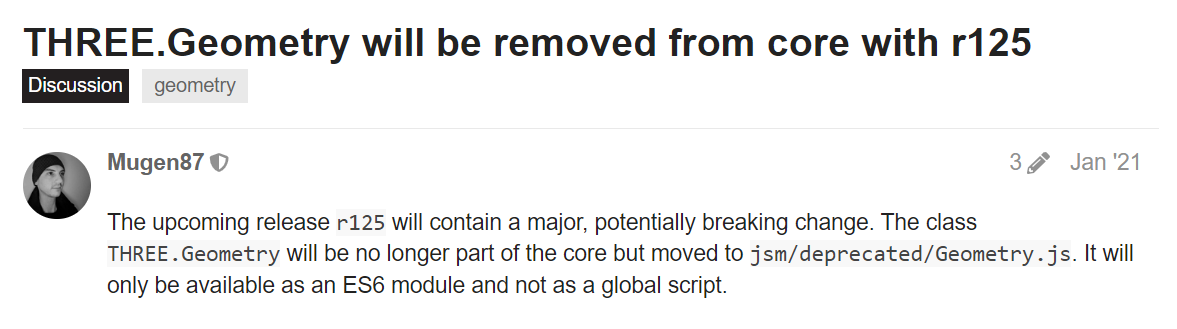
\includegraphics[width=1\textwidth]{images/three-deprecated.png}
        \pause \\ 
        $\xrightarrow{}$Decided to rewrite whole functionality
    \end{exampleblock}
\end{frame}

\begin{frame}
    \begin{exampleblock}{Advancements after rewrite}
        \begin{itemize}[label=-]
            \item New security requirements of JavaScript and modern browsers: need to load the code from some server $\xrightarrow{}$ way smaller file sizes\\
                (for small examples 9kB vs. 539kB)
                \pause
            \item More efficient Animations, faster loading, lower memory usage
                \pause
            \item Also works for triangular complexes\\
            $\xrightarrow{}$Does not depend on umbrella condition for visualization\\
        \end{itemize}
    \end{exampleblock}
\end{frame}

\section{GAPic}
\begin{frame}
    Afterwards decided to roll this feature into new package: \\
    \begin{center}
        GAP \textbf{i}mage \textbf{c}reator    
    \end{center}
    \pause
    Goal is to divide up working with triangular complexes/simplicial surfaces in \texttt{SimplicialSurfaces} and to visualize them in \texttt{GAPic}.
\end{frame}

\begin{frame}
    \begin{exampleblock}{New features since creating \texttt{GAPic}}
        \begin{itemize}[label=-]
            \item Most settings available via GUI in real time \pause
            \item \texttt{normalsMaterial} for visualizing angles of faces\\
            $\xrightarrow{}$ maps colors of a face smoothly depending on the normal \pause
            \item Intersection planes\\
            $\xrightarrow{}$ allows seeing inside complexes \pause
            \item Parameterized coordinates \\
            $\xrightarrow{}$ allows coordinates to be defined as any equation JavaScript can evaluate
        \end{itemize}
    \end{exampleblock}
\end{frame}

\begin{frame}
    \begin{exampleblock}{Future plans}
        \begin{itemize}[label=-]
            \item Currently in beta\\
            $\xrightarrow{}$ need to finish manual \pause
            \item Partial rewrite with new data structure\\
            $\xrightarrow{}$ will reduce storage especially for big animations
            \item Add library of often used coordinates \\
            $\xrightarrow{}$ e.g. icosahedra of length $1$\cite{ico}\pause
            \item Make compatible with objects from other packages\\
            $\xrightarrow{}$ e.g. \texttt{simpcomp} package or \pause\textbf{your package?}
        \end{itemize}
    \end{exampleblock}
\end{frame}

\begin{frame}
    \begin{center}
        \textbf{Time for Demonstrations}
    \end{center}
    \pause
    \bigskip
    \begin{itemize}[label=-]
        \item Triangular complex
        \item Improved performance
        \item Normals material
        \item Intersection planes
        \item Parameterized coordinates
    \end{itemize}
\end{frame}

\begin{frame}
    \textbf{\Large Thank you for your attention}\\ 
    \bigskip
    Want to get involved? $\xrightarrow{}$ \url{github.com/GAP-ART-RWTH/GAPic}\\
    \bigskip
    References:\\
    \printbibliography
\end{frame}

\end{document}
